\section{Running Example}
\label{sec:example}

%\begin{figure*}
%\begin{center}
%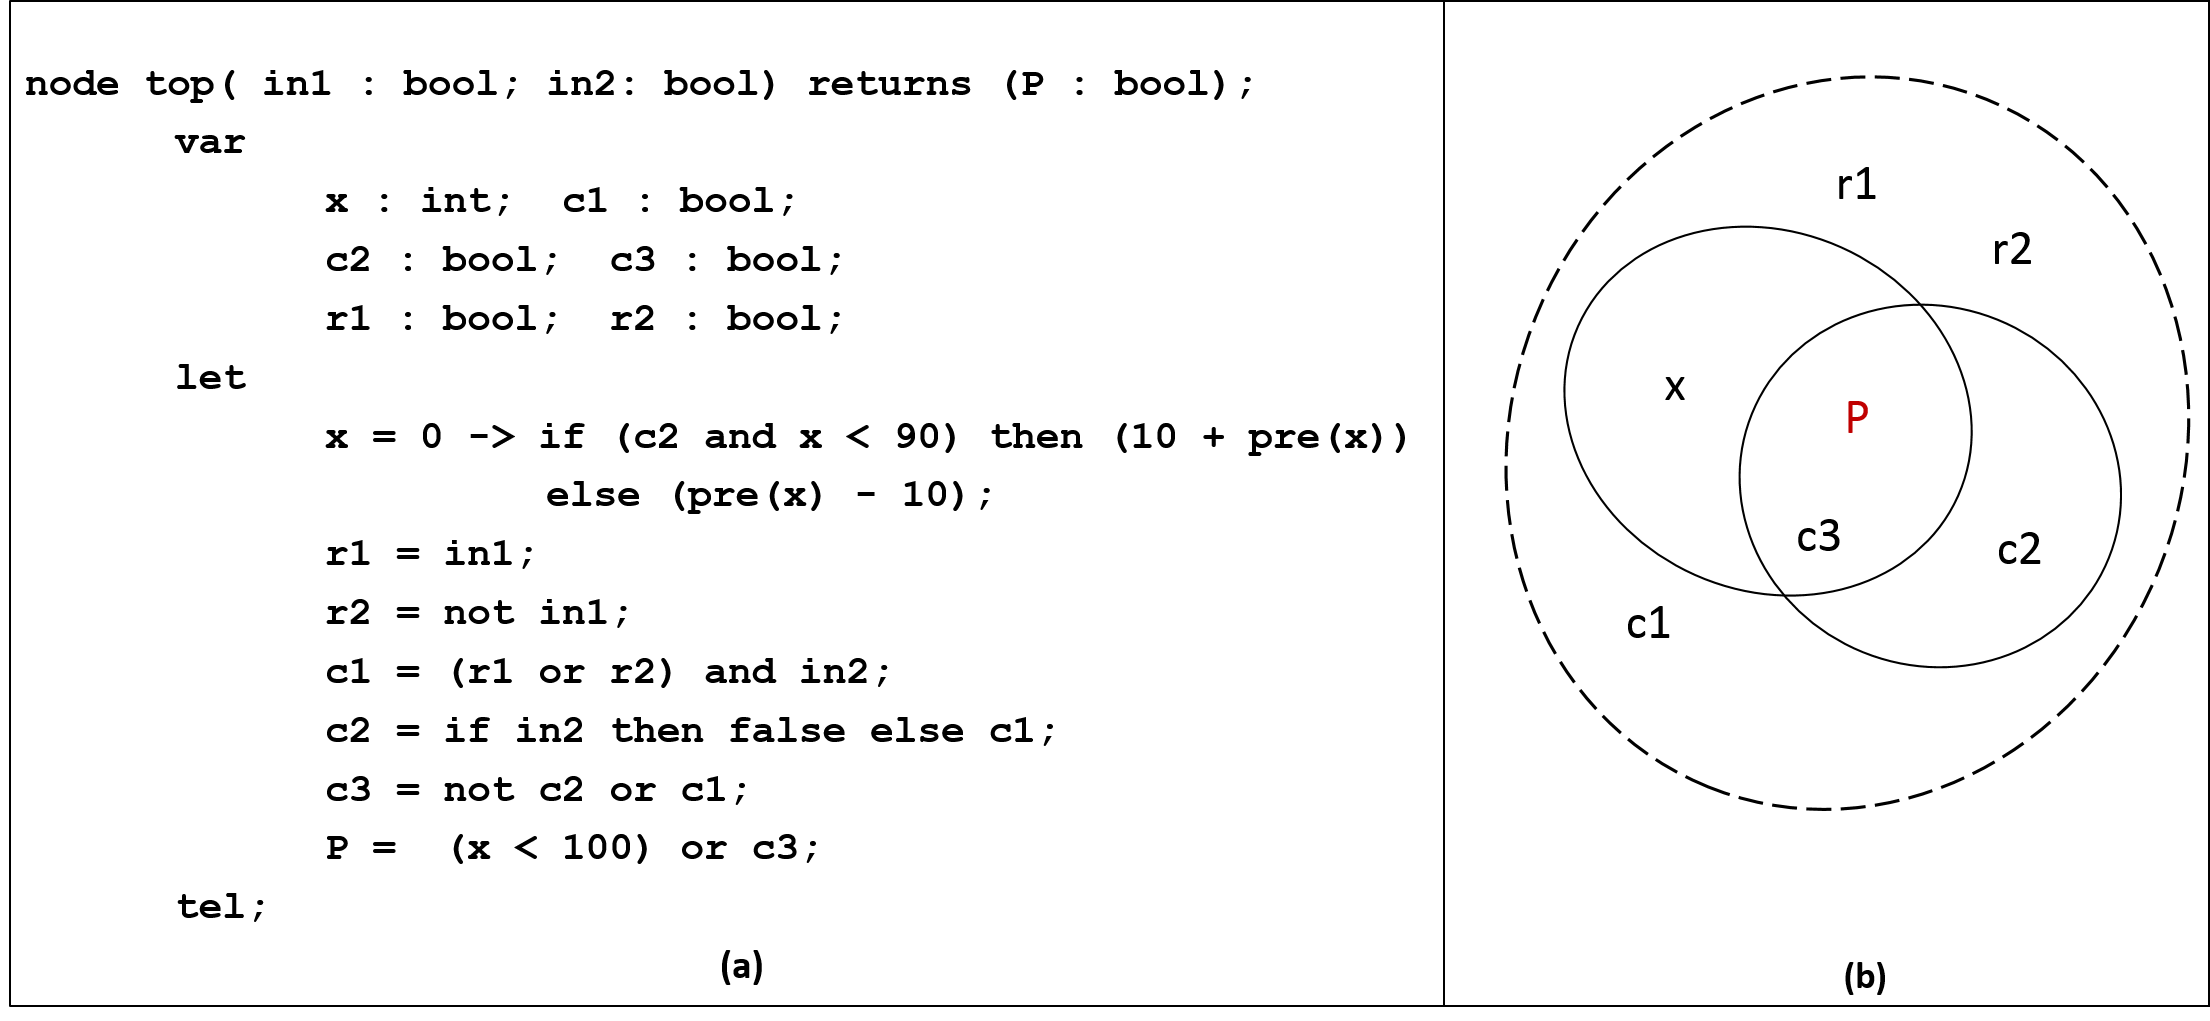
\includegraphics[width=0.8\textwidth]{figs/ex.png}
%\vspace{-0.1in}
%\caption{A Lustre model with property $P$}
%\label{fig:ex}
%\end{center}
%\end{figure*}

%% We put the image here so it shows up side-by-side with fig:ex-after
\begin{figure}
\centering

\includegraphics[width=0.85\columnwidth]{figs/aswcode.png}
\vspace{-0.1in}
\caption{Altitude Switch Model }
\label{fig:asw}
%\vspace{-0.2in}
\end{figure}

We will use a very simple system from the avionics domain to illustrate our approach. An Altitude Switch (ASW) is a hypothetical device that turns power on to another subsystem, the Device of Interest (DOI), when the aircraft descends below a threshold altitude and turns the power off again after we ascend over the threshold plus some hysteresis factor.  An implementation of an ASW containing two altimeters written in the Lustre language (simplified and adapted from~\cite{HCW02:ase-deviation}) is shown in Fig.~\ref{fig:asw}.  If either altimeter is below the constant {\small \texttt{THRESHOLD}}, then it turns on the DOI; else, if the system is inhibited or both altimeters are above the threshold plus the hysteresis factor {\small \texttt{T\_HYST}}, then the DOI is turned off, and if neither condition holds, then in the initial computation it is false and thereafter retains its previous value.  The notation {\small \texttt{(false -> pre(doi\_on))}} in equation (7) describes an initialized register in Lustre: in the first step, the expression is {\small \texttt{false}}, and thereafter it is the previous value of {\small \texttt{doi\_on}}.

A simple property {\small \texttt{on\_p}} states that if both altimeters are under the threshold, then the DOI is turned on.  This property can easily be proved over the model using a $k$-induction based verifier such as \texttt{JKind}~\cite{jkind}.


